\chapter{Fortgeschrittene Datenstrukturen}

Wir werden uns in diesem Kapitel mit Prioritätslisten beschäftigen. Es gibt noch viele weitere fortgeschrittene Datenstrukturen, z.B.
\begin{itemize}
  \item monotone ganzzahlige Prioritätslisten (später im Kapitel ``kürzeste Wege'')
  \item perfektes Hashing
  \item Suchbäume mit fortgeschrittenen Operationen
  \item externe Prioritätslisten (später im Kapitel ``Externe Algorithmen'')
  \item Geometrische Datenstrukturen (siehe Kapitel ``Geometrische Algorithmen'')
\end{itemize}

\section{Adressierbare Prioritätslisten}

Eine \term{adressierbare Prioritätsliste}\index{Adressierbare Prioritätsliste} muss folgende Funktionen implementieren:

\begin{pseudocode}
  \begin{tabular}{ll}
    \textbf{\textsc{build}}\( (\left \{ e_1,\dots,e_n \right \}) \) & \( M \coloneqq \left \{ e_1,\dots,e_n \right \} \) \\
    \textbf{\textsc{size}} & \textbf{return} \( \left\vert M \right\vert \) \\
    \textbf{\textsc{insert}}\( (e) \) & \( M \coloneqq M \cup \left \{ e \right \} \) \\
    \textbf{\textsc{min}} & \textbf{return} \( \min M \) \\
    \textbf{\textsc{deleteMin}} & \( e \coloneqq \min \); \enskip{} \( M \coloneqq M \setminus \left \{ e \right \} \); \enskip{} \textbf{return} \( e \) \\
    \textbf{\textsc{remove}}\( (h : \text{Handle}) \) & \( e \coloneqq h \); \enskip{} \( M \coloneqq M \setminus \left \{ e \right \} \); \enskip{} \textbf{return} \( e \) \\
    \textbf{\textsc{decreaseKey}}\( (h : \text{Handle}, k : \text{Key}) \) & \( \text{key}(h) \coloneqq k \) \\
    \textbf{\textsc{merge}}\( (M') \) & \( M \coloneqq M \cup M' \)
  \end{tabular}
\end{pseudocode}

Adressierbare Prioritätslisten haben viele Anwendungen, beispielsweise im \emph{Dijkstra-Algorithmus} für kürzeste Wege oder in der Graphpartitionierung. Allgemein lassen sich adressierbare Prioritätslisten gut bei Greedy-Algorithmen verwenden, bei denen sich die Prioritäten (begrenzt) ändern.

\subsection{Datenstruktur}

Als grundlegende Datenstruktur wird ein Wald heap-geordneter Bäume verwendet. Hier wird also der Binary Heap verallgemeinert
\begin{itemize}
  \item Baum \( \to \) Wald
  \item zwei Kindknoten \( \to \) beliebig viele Kindknoten
\end{itemize}

Wir verwenden folgende grundlegende Operationen zur Bearbeitung solcher Wälder:
\begin{itemize}

  \begin{minipage}{.475\textwidth}
    \item \textbf{cut}: Teilbaum ausschneiden und als neuen Baum speichern
  \end{minipage}
  \hfill
  \begin{minipage}{.475\textwidth}
    \begin{figure}[H]
      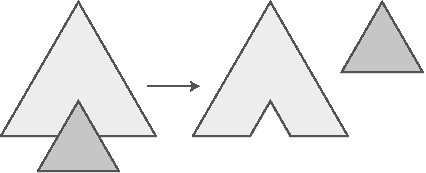
\includegraphics[width=0.8\textwidth]{Cut}
    \end{figure}
  \end{minipage}

  \begin{minipage}{.475\textwidth}
    \item \textbf{link}: Baum 2 mit größerem Wurzelknoten als Baum 1 an Baum 1 als Kindknoten des Wurzelknotens anhängen
  \end{minipage}
  \hfill
  \begin{minipage}{.475\textwidth}
    \begin{figure}[H]
      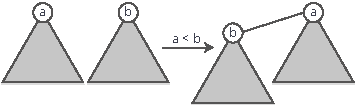
\includegraphics[width=\textwidth]{Link}
    \end{figure}
  \end{minipage}

  \item \textbf{union}: \( \text{union}(a,b) = \text{link}(\min(a,b), \max(a,b)) \)
\end{itemize}

\subsection{Dijkstras Algorithmus}

\term{Dijkstras Algorithmus}\index{Dijkstras Algorithmus} kann die Distanz zwischen einem Startknoten \( s \) und jedem anderen Knoten des Graphen berechnen.

\begin{pseudocode}
  \textbf{\textsc{Dijkstra}}\( (s : \text{Node}, T : \text{Tree}) \) \\
  \textcolor{gray}{// Initialisieren: Distanz zu jedem Knoten ist \( \infty \), zu Startknoten \( 0 \).} \\
  \( d = \left\langle \infty,\ldots,\infty \right\rangle \) \\
  \( d[s] = 0 \) \\
  \textcolor{gray}{// Startknoten zu PQ hinzufügen.} \\
  \( Q\text{.insert}(s) \) \\
  \textbf{while} \( Q \neq \varnothing \) \textbf{do} \\
  \phantom{\enskip} \( u \coloneqq Q\text{.deleteMin} \) \\
  \phantom{\enskip} \textbf{for all} \( (u,n) \in E \) \textbf{do} \\
  \phantom{\enskip} \phantom{\enskip} \textbf{if} \( n \not \in Q \) \textbf{then} \( Q\text{.insert}(n) \) \\
  \phantom{\enskip} \phantom{\enskip} \textbf{if} \( d[n] > d[u] + c(u,n) \) \textbf{then} \( d[n] = d[u] + c(u,n) \) \\
\end{pseudocode}

\section{Pairing Heaps}

\term{Pairing Heaps}\index{Pairing Heaps} müssen folgende Funktionen implementieren:
\begin{pseudocode}
  \textbf{\textsc{insertItem}}\( (h: \text{Handle}) \) \\
  \phantom{\enskip} \( \text{newTree}(h) \) \\
  \textbf{\textsc{newTree}}\( (h: \text{Handle}) \) \\
  \phantom{\enskip} \( \text{forest} \coloneqq \text{forest} \cup \left \{ h \right \} \) \\
  \phantom{\enskip} \textbf{if} \( \ast h < \min \) \textbf{then} \( \text{minPtr} \coloneqq h \) \\
  \textbf{\textsc{decreaseKey}}\( (h : \text{Handle}, k : \text{Key}) \) \\
  \phantom{\enskip} \( \text{key}(h) \coloneqq k \) \\
  \phantom{\enskip} \textbf{if} \( h \) not a root \textbf{then} \( \text{cut}(h) \) \textbf{else} \( \text{updateMinPtr}(h) \) \\
  \textbf{\textsc{deleteMin}}\( () : \text{Handle} \) \\
  \phantom{\enskip} \( m \coloneqq \text{minPtr} \) \\
  \phantom{\enskip} \( \text{forest} \coloneqq \text{forest} \setminus \left \{ m \right \} \) \\
  \phantom{\enskip} \textbf{foreach} child \( h \) of \( m \) \textbf{do} \( \text{newTree}(h) \) \\
  \phantom{\enskip} pairwiseRootUnion\( () \) \\
  \phantom{\enskip} updateMinPtr\( () \) \\
  \phantom{\enskip} \textbf{return} \( m \) \\
  \textbf{\textsc{pairwiseRootUnion}}\( () \) \\
  \phantom{\enskip} \textcolor{gray}{// see picture} \\
  \textbf{\textsc{merge}}\( (o: \text{AdressablePQ}) \) \\
  \phantom{\enskip} \textbf{if} \( \ast\text{minPtr} > \ast(o\text{.minPtr}) \) \textbf{then} \( \text{minPtr} \coloneqq o\text{.minPtr} \) \\
  \phantom{\enskip} \( \text{forest} \coloneqq \text{forest} \cup o\text{.forest} \) \\
  \phantom{\enskip} \( o\text{.forest} \coloneqq \varnothing \)
\end{pseudocode}

Einige Funktionalitäten lassen sich gut veranschaulichen:

\begin{minipage}{.475\textwidth}
  \begin{figure}[H]
    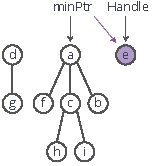
\includegraphics[width=0.5\textwidth]{NewTree}
    \caption{\code{newTree}: Element \( e \) wird hinzugefügt (ggf.\ auch ein ganzer Baum) und --- falls nötig --- der \code{minPtr} angepasst}
  \end{figure}
\end{minipage}
\hfill
\begin{minipage}{.475\textwidth}
  \vspace{1cm}
  \begin{figure}[H]
    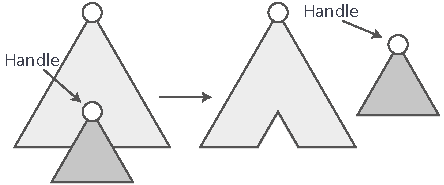
\includegraphics[width=\textwidth]{DecreaseKey}
    \caption{\code{decreaseKey}: Durch Herabsetzen des Keys wird eventuell die Heap-Eigenschaft verletzt, deswegen wird der Teilbaum ausgeschnitten und als neuer Baum hinzugefügt}
  \end{figure}
\end{minipage}

\begin{figure}[H]
  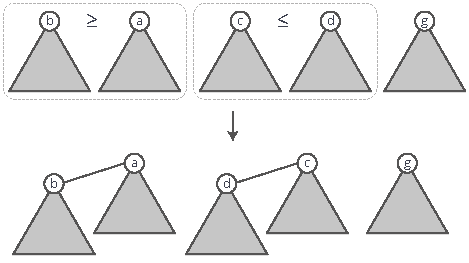
\includegraphics[width=0.6\textwidth]{PairWiseRootUnion}
  \caption{\code{pairwiseRootUnion} fügt jeweils zwei Bäume des Waldes zu einem größeren Baum zusammen, indem die beiden Wurzeln miteinander verglichen werden und eine der beiden Wurzeln Kindknoten der anderen wird}
\end{figure}

\subsection{Repräsentation}

Meistens speichert man Pairing Heaps als doppelt verkettete Liste der Wurzeln. Die Baum-Items können beispielsweise folgendermaßen gespeichert werden:

\begin{figure}[H]
  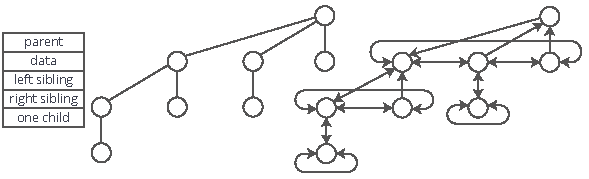
\includegraphics[width=0.8\textwidth]{PairingHeapRepresentation}
  \caption{Speichern der Baum-Items. Man kann hier noch Speicherplatz einsparen, indem man \emph{left sibling} und \emph{parent} zusammenfasst. Allerdings muss man dann alle Geschwisterknoten traversieren, damit man zum Elternknoten kommen kann, da nur der linkeste Kindknoten den Elternknoten speichert}
\end{figure}

\subsection{Analyse}

\begin{itemize}
  \item \code{insert} und \code{merge} gehen in \( O(1) \).
  \item \code{deleteMin} und \code{remove} gehen jeweils in \( O(\log n) \) amortisiert.
  \item \code{decreaseKey} ist schwieriger zu analysieren, geht aber amortisiert in \( O(\log\log n) \leq T \leq O(\log n) \) und ist in der Praxis sehr schnell.
\end{itemize}

Wir werden als nächstes \emph{Fibonacci-Heaps} verwenden, um noch mehr Leistung rauszukitzeln.

\section{Fibonacci-Heaps}

Mithilfe von Fibonacci-Heaps erhalten wir eine amortisierte Komplexität von \( O(\log n) \) für \code{deleteMin} und \( O(1) \) für alle anderen Operationen.

Fibonacci-Heaps speichern ein paar Zusatzinformationen pro Knoten ab, wodurch neue Hilfsfunktionen kreiert werden können, die diese Beschleunigung ermöglichen:

\begin{itemize}
  \item \textbf{Rank} eines Knotens: Anzahl direkter Kinder
  \item \textbf{Mark}: Knoten, die ein Kind verloren haben, werden markiert
  \item \textbf{Vereinigung nach Rank}: Union nur für gleichrangige Wurzeln
  \item \textbf{Kaskadierende Schnitte}: Knoten, die beide markiert sind (also ein Kind verloren haben), werden geschnitten
\end{itemize}

\subsection{Repräsentation}

\begin{minipage}{.725\textwidth}
  Die Repräsentation ist analog zu der von Pairing Heaps, die Wurzeln werden wieder als doppelt verkettete Liste gespeichert und die Baum-Items als Parameterliste:
\end{minipage}
\hfill
\begin{minipage}{.25\textwidth}
  \begin{figure}[H]
    \begin{tabular}{| c |}
      \hline
      parent \\
      \hline
      data, \emph{rank}, \emph{mark} \\
      \hline
      left sibling \\
      \hline
      right sibling \\
      \hline
      one child \\
      \hline
    \end{tabular}
  \end{figure}
\end{minipage}

\subsection{Funktionalität}

\code{insert} und \code{merge} werden wie gehabt implementiert. \code{decreaseKey} verwendet die neue \code{cascadingCut}-Methode und \code{deleteMin} Union-by-Rank. Wir beschleunigen Union-by-Rank, indem wir ein Feld pro Rank bereitstellen und Knoten in diese Felder eintragen. Sollte das passende Feld bereits belegt sein, so wird der neue Knoten mit dem Knoten, der sich im Feld befindet gelinkt und entsprechend verschoben.

\begin{minipage}{.625\textwidth}
  \begin{pseudocode}
    \textbf{\textsc{deleteMin}}\( () : \text{Handle} \) \\
    \phantom{\enskip} \( m \coloneqq \text{minPtr} \) \\
    \phantom{\enskip} \( \text{forest} \coloneqq \text{forest} \setminus \left \{ m \right \} \) \\
    \phantom{\enskip} \textbf{foreach} child \( h \) of \( m \) \textbf{do} \( \text{newTree}(h) \) \\
    \phantom{\enskip} \textbf{while} \( \exists \ a,b \in \text{forest} : \text{rank}(a) \equiv \text{rank}(b) \) \textbf{do} \\
    \phantom{\enskip} \phantom{\enskip} \( \text{union}(a,b) \) \\
    \phantom{\enskip} \( \text{updateMinPtr}() \) \\
    \phantom{\enskip} \textbf{return} \( m \) \\
    \textbf{\textsc{decreaseKey}}\( (h: \text{Handle}, k : \text{Key}) \) \\
    \phantom{\enskip} \( \text{key}(h) \coloneqq k \) \\
    \phantom{\enskip} \( \text{cascadingCut}(h) \) \\
    \textbf{\textsc{cascadingCut}}\( h : \text{Handle} \) \\
    \phantom{\enskip} \textbf{assert} \( h \) is not a root \\
    \phantom{\enskip} \( p \coloneqq \text{parent}(h) \) \\
    \phantom{\enskip} \( \text{unmark}(h) \) \\
    \phantom{\enskip} \( \text{cut}(h) \) \\
    \phantom{\enskip} \textbf{if} \( p \) is marked \textbf{then} \\
    \phantom{\enskip} \phantom{\enskip} \( \text{cascadingCut}(p) \) \\
    \phantom{\enskip} \textbf{else} \( \text{mark}(p) \)
  \end{pseudocode}
  
  Eine amortisierte Analyse von \code{deleteMin} ergibt \( \Omega(\log n) \) für vergleichsbasiertes \code{deleteMin}.
\end{minipage}
\hfill
\begin{minipage}{.35\textwidth}
  \begin{figure}[H]
    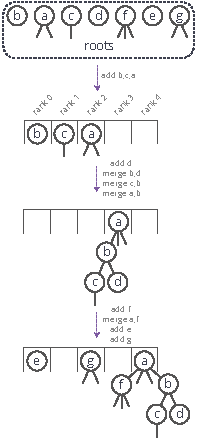
\includegraphics[width=\textwidth]{FastUnionByRank}
    \caption{Fast Union-by-Rank}
  \end{figure}
\end{minipage}